\documentclass[12pt]{report}			% Začátek dokumentu
\usepackage{SP}							% Import stylu

\author{Jonáš Havelka}
\title{Neuronové sítě}
\date{19. února 2020}
\vedouci{Dr. rer. nat. Michal Kočer}
\place{V~Českých Budějovicích}
\skolnirok{2019/2020}
\logo{
\includegraphics[scale=0.75]{logo_gymji.jpg}}

\sloppy

\newcommand{\Kotlin}{\icon{Kotlin-logo.png}\gls{Kotlin}}
\newcommand{\git}{\underlineicon{Git-logo.png}\,git}
\newcommand{\GitHub}{\bigunderlineicon{GitHub-logo.png}\,GitHub}
\newcommand{\Gradle}{\bigicon{Gradle-logo.png}Gradle}

\newcommand{\R}{\mathbb{R}}   			% množina reálnách čísel
\newcommand{\Z}{\mathbb{Z}}   			% množina celých čísel
\newcommand{\N}{\mathbb{N}}   			% množina přirozených čísel
\newcommand{\powerset}[1]{\mathcal{P} ( #1 )}   
										% potenční množina -- množina všech podmnožin
										
\usepackage{fancyvrb}					% balíček pro použití verbatim v poznámkách pod čarou
\usepackage{subcaption}					% balíček pro figuru s více obrázky
\usepackage{forest}						% balíček pro kresbu diagramů
\VerbatimFootnotes

\newcommand{\W}{\mathbb{W}}

\usepackage{listings}

\lstdefinelanguage{Kotlin}{
  comment=[l]{//},
  commentstyle={\color{gray}\ttfamily},
  emph={delegate, filter, first, firstOrNull, forEach, lazy, map, mapNotNull, println, return@},
  emphstyle={\color{OrangeRed}},
  identifierstyle=\color{black},
  keywords={abstract, actual, as, as?, break, by, class, companion, continue, data, do, dynamic, else, enum, expect, false, final, for, fun, get, if, import, in, interface, internal, is, null, object, override, package, private, public, return, set, super, suspend, this, throw, true, try, typealias, val, var, vararg, when, where, while},
  keywordstyle={\color{NavyBlue}\bfseries},
  morecomment=[s]{/*}{*/},
  morestring=[b]",
  morestring=[s]{"""*}{*"""},
  ndkeywords={@Deprecated, @JvmField, @JvmName, @JvmOverloads, @JvmStatic, @JvmSynthetic, Array, Byte, Double, Float, Int, Integer, Iterable, Long, Runnable, Short, String},
  ndkeywordstyle={\color{BurntOrange}\bfseries},
  sensitive=true,
  stringstyle={\color{ForestGreen}\ttfamily},
}

\lstset{language=Kotlin, breaklines=true, postbreak=\mbox{\textcolor{red}{$\hookrightarrow$}\space}, basicstyle=\tiny}
\newcommand{\KotlinCode}[1]{\addcontentsline{toc}{subsection}{#1}\lstinputlisting[caption={#1}, label={lst:#1}]{appendixFiles/#1}}

\usepackage{tikz}
\usetikzlibrary{calc}
\tikzset{X/.style={circle,thick,draw}}
\tikzset{S/.style={thick,draw, minimum size=1cm}}

\usepackage{pgfplots}
\pgfplotsset{compat=1.11}

\pgfplotsset{every tick label/.append style={font=\scriptsize}}
\newcommand{\drawF}[2]{
	\begin{axis}[grid=both,
          		xmax=4,ymax=2,xmin=-4,ymin=-2,
	     		axis lines=middle,
         		enlargelimits,
         		scale=0.7]
		\addplot[thick, blue, samples=100, #1] {#2};
	\end{axis}
}

\tikzset{
    binaryStep/.pic={
        \drawF{samples=400}{abs(x)/(2*x) + 0.5}
    },
    identity/.pic={
        \drawF{}{x}
    },
    sigmoid/.pic={
    	\drawF{}{1/(1+e^-x)}
    },
    tanh/.pic={
    	\drawF{}{tanh(x)}
    },
    swish/.pic={
    	\drawF{}{x/(1+e^-x)}
    },
    rectifiedLinearUnit/.pic={
        \drawF{samples=400}{x^2/(2*abs(x)) + x*0.5}
    },
    leakyRectifiedLinearUnit/.pic={
        \drawF{samples=400}{x^2/(2*abs(x)) + x*0.5 + 0.1*(x^2/(-2*abs(x)) + x*0.5)}
    },
    hardHyperbolicFunction/.pic={
    	\drawF{samples=400}{abs(x-1)/(2*(x-1)) - abs(-x-1)/(2*(-x-1)) + (abs(-x+1)/(2*(-x+1)) + 0.5)*(abs(x+1)/(2*(x+1)) + 0.5)*x}
    },
    softPlus/.pic={
    	\drawF{}{ln(1+e^x)}
    },
    softSign/.pic={
    	\drawF{}{x/(abs(x)+1)}
    },
    sin/.pic={
    	\drawF{}{sin(deg(x))}
    }
}
   
\newcommand{\figF}[2]{
	\begin{figure}[h]
		\centering
	  	\tikz \pic{#1};
		\caption{#2}
	\end{figure}
} 
   
\newcommand{\figSF}[2]{
	\begin{subfigure}[b]{0.3\textwidth}
		\centering
	  	\tikz \pic{#1};
		\caption{#2}
	\end{subfigure}
} 
	
	\newcommand{\delete}[1]{}				    	    

\addto\captionsczech{\renewcommand{\figurename}{Obr.}}

\newcommand{\glsref}[1]{\glsdisp{#1}{\phantom{}}}

\begin{document}

	\mytitlepage						% Vygenerování titulní strany
	
	\prohlaseni{
		Prohlašuji, že jsem tuto práci vypracoval samostatně s~vyznačením všech použitých pramenů.
	}	
	
	\abstrakt{
	
		Neuronové sítě se dnes objevují všude, ať už jde o~vyhledávání, překládání nebo třeba jen zpracovávání dat. Mnoho programovacích jazyků má své knihovny pro práci s~umělou inteligencí, ale právě \Kotlin{}, který je mým oblíbeným programovacím jazykem a~který lze použít skoro kdekoliv (webové stránky, servery, mobily), takovou knihovnu postrádá. Proto jsem se rozhodl svoji práci koncipovat jako snahu o~implementování takové knihovny.
		% Abstrakt
	}{
		Neuronové sítě, Neuron, Umělá inteligence, Aktivační funkce, \Kotlin, Multiplatformní knihovna, Java, Javascript						% Klíčová slova
	}
	
	\podekovani{
		Poděkování patří hlavně mému učiteli informatiky, který je zároveň vedoucím mé práce, za skvělou výuku na hodinách a~velkou trpělivost při kontrole našich prací. Také nesmím zapomenout na Alžbětu Neubauerovou, která mě celý rok podporovala a~několikrát provedla korekturu mé práce.
		
		Dále bych rád poděkoval všem komunitám, jejichž nástroje jsem používal, tj.~\mbox{JetBrains}, v~jejichž programovacím jazyce \Kotlin{} programuji a~jejichž prostředí IntelliJ k~tomu využívám, \Gradle{}, který používám ke kompilaci, \LaTeX{}, ve kterém píšu text, a~dále \git{} a~\GitHub{}, jež uchovávají má data, ať už text nebo knihovnu. 					% Poděkování
	}
	
	\tableofcontents\newpage			% Obsah
	
	
	
	
	\chapter*{Úvod}
	
		Neuronové sítě jsou v~poslední době velmi skloňované téma. Nikdo pořádně neví, jak to, že fungují tak dobře. Cílem této práce však nebude zkoumat neuronové sítě, ale implementovat je v~co největším rozsahu (ať už struktury bez širšího využití jako asociativní paměť, nebo často používané konvoluční sítě na rozpoznávání obrázků).
		
		\gls{Kotlin} je ideální programovací jazyk pro vývoj knihovny, protože je interoperabilní s~Javou, Javascriptem i~C, a~tak umožňuje tuto knihovnu používat jak pro \gls{JVM} (Java Virtual Machine), tak i~v~prohlížeči nebo v~programech kompilovaných přímo do binárního kódu.
		
		V~textu jsou použity pojmy ze stavby biologického neuronu, objektově orientovaného programování, \gls{Kotlin}u, atd. Tyto pojmy jsou vysvětleny na konci práce. 
		
		Celá maturitní práce je k~dispozici na GitHubu, text včetně zdrojového LaTeXu na adrese \url{https://github.com/JoHavel/Maturitni-Seminarni-Prace/tree/my\_work} a~knihovna samotná pak na \url{https://github.com/JoHavel/NeuralNetwork}.
	
	
	\part{Teoretická část}
		
			\chapter{Laický náhled na neuronové sítě}
			
				\section{Neuron}
					Počítačové neuronové sítě nejsou jen výmysl lidí, jejich základ nalezneme v~nervových soustavách živočichů. Základní stavební jednotka takové soustavy (stejně tak i~neuronové sítě) je \emph{neuron}. Neuron funguje tak, že přes \emph{\gls{dendrit}y} přijímá elektrické (přesněji iontové) signály od jiných neuronů a~když součet signálů přeteče určitou danou \emph{mez}, vyšle neuron signál přes \emph{\gls{axon}y} dál do dalších neuronů.
					
					Přenos signálu z~\gls{axon}u do \gls{dendrit}u se odehrává v~malých prostorách mezi nimi zvaných \emph{\gls{synapse}}. Vodivost synapsí je ovlivněna jejich chemickým složením, a~proto se domníváme, že proces učení probíhá měněním těchto chemických spojů \autocite[s. 491]{book:Informatika}.
					
					Náš umělý neuron tedy bude mít \emph{seznam \gls{dendrit}ů} (nesoucích informaci z~jakého neuronu vedou signál a~jak ho mění \gls{synapse}), tzv.~\emph{aktivační funkci} (viz dále) a~výstupní signál. Často navíc bude obsahovat základní hodnotu (angl. \emph{bias}), která reprezentuje mez, při jejímž překročení začne neuron vysílat signál. Jinak řečeno posouvá aktivační funkci ve směru osy~$x$.
					
					Neuron (hlavně ten umělý) ilustruje obrázek~\ref{fig:neuron} nacházející se v~další kapitole. Podrobněji o~souvislosti biologických a~umělých neuronových sítích pojednává \autocite{book:BNN}.
				
				\section{Aktivační funkce}
					Jak už bylo zmíněno, přírodní neuron funguje na principu toho, že když součet vstupních signálů nepřekračuje určitou mez, nevysílá neuron žádný (nebo téměř žádný) signál. Když je však tato mez překonána, neuron vyšle signál. V~podstatě tedy vysílá buď 0 nebo 1. Pro účely umělého neuronu je 0 a~1 nedostačující, jelikož při procesu učení potřebujeme měnit hodnoty jemně, abychom nerozbili již naučené znalosti.
					
					Proto se jako aktivační funkce (tedy to, co určuje jaký má být výstup v~závislosti na součtu vstupů, v~případě přírody tedy funkce zobrazující interval $-\infty$ až mez (bias) na 0 a~zbylá čísla na 1 viz \emph{binární krok} v~sekci~\ref{s:af}) používají funkce co nejvíce podobné právě tomuto binárnímu kroku, které jsou ale spojité a~mají co \uv{nejhezčí} derivace (protože při zpětné propagaci právě podle derivace určíme, jak moc daný neuron ovlivňuje výsledek).
				
				\section{Sítě} \label{s:net}
					Jelikož \uv{nahodilé neurony} by se těžko udržovaly v~paměti a~operace na nich by byly velmi pomalé, potřebujeme síť nějak uspořádat. Nejjednodušším uspořádáním jsou \emph{vrstvy} (viz obrázek~\ref{fig:bnn}). Každý neuron z~jedné vrstvy má \gls{dendrit}y ze všech neuronů z~vrstvy minulé. Tak se předejde \glsdisp{cyklus}{cyklům}, které jsou složité na výpočty, a~navíc si nemusíme u~každého neuronu pamatovat, ze kterých neuronů do něj vede signál.
					
					Velmi využívanými strukturami jsou také konvoluční neuronové sítě, kde nejdříve aplikujeme filtry\footnote{Často malé neuronové sítě, které sami vytvoříme. Sítě používané jako filtry se nemusí učit (učení filtrů není vzhledem k~obtížnosti zatím implementováno). Další možný filtr je třeba Fourierova transformace viz \autocite{art:FCNN}, kterou se však dále zabývat nebudeme (tato možnost není ani implementována v~knihovně).} na části vstupních dat a~teprve výstupy z~těchto filtrů jsou vstupem do neuronové sítě. O~konvolučních sítích se můžete dočíst v~\autocite{lec:CNN} nebo v~\autocite{sem:CNN}.
					
					I~tak se \uv{nahodilé neurony} občas používají, jelikož při malém množství neuronů a~hlavně při malém množství synapsí je přepočítání samotných neuronů efektivnější než počítání celých vrstev. Ukázkou takové malé sítě je asociativní paměť, kde neuronům přiřadíme objekty, které si tato síť má \uv{pamatovat}. Když chceme zjistit, co je v~paměti asociováno s~daným objektem, vybudíme (v~umělé síti to znamená nastavíme výstupní signál na 1) neuron odpovídající tomuto objektu a~následně sledujeme, které další neurony jsou vybuzeny (viz obrázek~\ref{fig:am}). Takto funguje i~lidská paměť, pamatujeme si právě asociace. Umělou asociativní paměť zmiňuje \autocite{book:Informatika}.
					
					\begin{figure}[h]
						\resizebox{\textwidth}{!}{%
							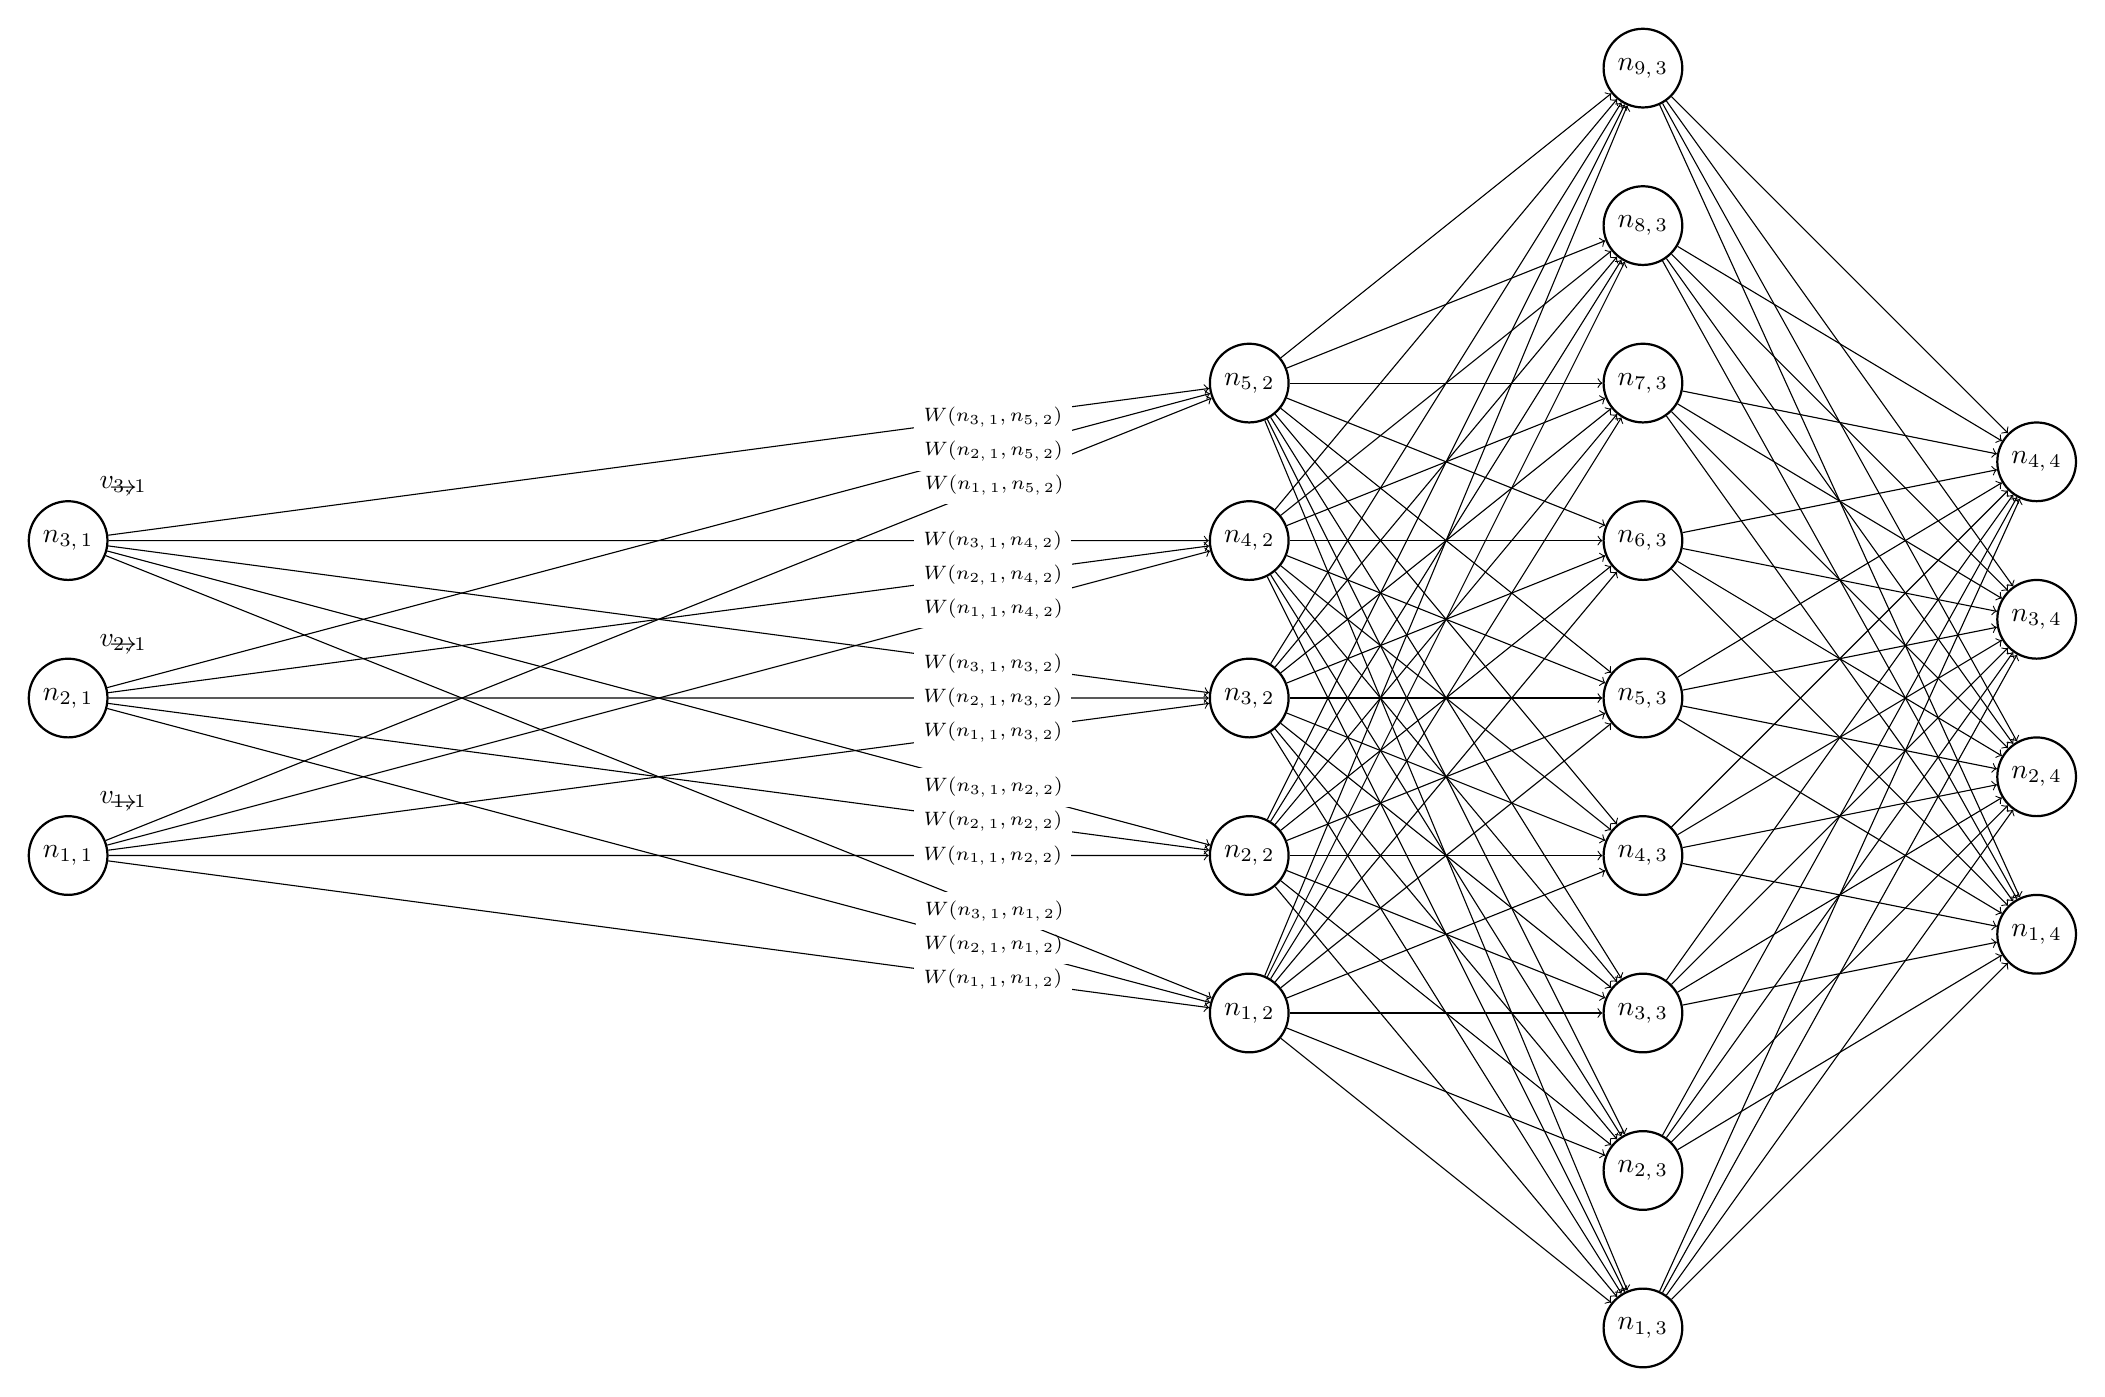
\begin{tikzpicture}
								\def\first{3}
								\def\second{5}
								\def\third{9}
								\def\fourth{4}
								\foreach \x in {1,...,\first}{%
							    	\node[X] (A\x) at (0, 2*\x-\first) {$n_{\x,\,1}$};
							    	\node[align=center] at ($(A\x)+(0.7,0.7)$) {$v_{\x,\,1}$\\[-3.5mm] $\rightarrow$};
							    }
     
								\foreach \x in {1,...,\second}{%
					    	  		\node[X] (B\x) at (15, 2*\x-\second) {$n_{\x,\,2}$};
								}
					     
								\foreach \x in {1,...,\third}{%
							    	\node[X] (C\x) at (20, 2*\x-\third) {$n_{\x,\,3}$};
							    }
				     
								\foreach \x in {1,...,\fourth}{%
							    	\node[X] (D\x) at (25, 2*\x-\fourth) {$n_{\x,\,4}$};
							    }
     
					    		\foreach \x in {1,...,\first}{%
					    			\foreach \y in {1,...,\second}{%
						    		\draw [->] (A\x) -- ($(A\x)!.6!(B\y)$) -- node[fill=white] {\scriptsize $\W(n_{\x,\,1}, n_{\y,\,2})$} (B\y);
					    			}
							    }
     
							    \foreach \x in {1,...,\second}{%
					    			\foreach \y in {1,...,\third}{%
								    	\draw [->] (B\x) -- (C\y);
			    					}
						    	}
	     
							    \foreach \x in {1,...,\third}{%
					    			\foreach \y in {1,...,\fourth}{%
			    						\draw [->] (C\x) -- (D\y);
				    				}
							    }
						    \end{tikzpicture}
						}
						\caption{Běžná neuronová síť ($\W$ jsou váhy, $n$ neurony a~$v$ je výstupní signál, viz kapitola~\ref{s:fn}, konkrétně sekce~\ref{s:n})}
						\label{fig:bnn}
					\end{figure}
					
					
					\newcommand{\pictureAP}{
						\resizebox{\textwidth}{!}{%
							\begin{tikzpicture}  
								\node[X1] (winter) at (0, 0) {zima};
								\node[X2] (ice) at (2, 0) {led};
								\node[X2] (snow) at (2, 2) {sníh};
								\node[X3] (white) at (4, 0) {bílá};
								\node[X4] (black) at (4, 2) {černá};
								\node[X2] (summer) at (-2, -2) {léto};
								\node[X4] (color) at (4, -2) {barva};
								\node[XX] (apple) at (0, 2) {jablko};
								\node[XX] (fruit) at (-2, 2) {ovoce};
								\node[XX] (what) at (-2, 0) {kropáč};
								\node[XX] (red) at (2, -2) {červená};
								\node[XX] (car) at (0, -2) {auto};
								
								\draw[->] (winter) to[out=15,in=165] (ice);
								\draw[->] (ice) to[out=-165,in=-15] (winter);
								\draw[->] (winter) to[out=-120,in=30] (summer);
								\draw[->] (summer) to[out=60,in=-150] (winter);
								\draw[->] (snow) to[out=-120,in=30] (winter);
								\draw[->] (winter) to[out=60,in=-150] (snow);
								\draw[->] (apple) -- (fruit);
								\draw[->] (ice) -- (white);
								\draw[->] (snow) to[out=-30,in=120] (white);
								\draw[->] (white) to[out=150,in=-60] (snow);
								\draw[->] (white) to[out=105,in=-105] (black);
								\draw[->] (black) to[out=-75,in=75] (white);
								\draw[->] (red) -- (color);
								\draw[->] (white) -- (color);
								\draw[->] (black) to[out=-40,in=40] (color);
							
						    \end{tikzpicture}
						}
					}
					\newcommand{\subf}[1]{
						\begin{subfigure}[b]{0.45\textwidth}
							\pictureAP
							\caption{#1}
						\end{subfigure}
					}
					\begin{figure}
						\tikzset{XX/.style={X, minimum size=1.7cm}}
						\tikzset{X1/.style={XX}}
						\tikzset{X2/.style={XX}}
						\tikzset{X3/.style={XX}}
						\tikzset{X4/.style={XX}}
						\subf{Vybuzení 1. neuronu (zimy)}
						\tikzset{X1/.style={XX, color=red}}
						\subf{1 krok po vybuzení 1. neuronu}
						\tikzset{X2/.style={XX, color=red}}
						\subf{2 kroky po vybuzení 1. neuronu}
						\tikzset{X3/.style={XX, color=red}}
						\subf{3 kroky po vybuzení 1. neuronu}
						\tikzset{X4/.style={XX, color=red}}
						\subf{4 kroky po vybuzení 1. neuronu}
						\caption{Asociativní paměť, červeně jsou vybuzené neurony}
						\label{fig:am}
					\end{figure}
					
				\section{Dopředná propagace a~zpětná propagace}
					Dopředná propagace (častěji se používá anglický výraz forward propagation) je jednoduše spočítání signálů ve všech neuronech. Tedy u~každého neuronu se sečtou vstupní signály (popř. přičte bias) a~spočítá se funkční hodnota aktivační funkce v~tomto bodě.
					
					Naopak zpětná propagace (častěji se používá anglický výraz backward propagation či back\-propagation) je na základě chyby, kterou spočítáme z~výstupu neuronové sítě a~předpokládaného výstupu, určení, které proměnné hodnoty (\gls{synapse} a~biasy) se na ní nejvíce podílejí. Potom tyto hodnoty posuneme odpovídajícím způsobem (stejně jako příroda mění chemické vlastnosti \gls{synapse}). Z~matematického pohledu se hodnoty posunou proti směru \gls{gradient}u chyby, jelikož právě \gls{gradient} udává, kterým směrem máme souřadnice (tj.~váhy a~biasy) posunout, aby funkce (tj.~chyba) vzrostla.
					
				\section{Využití neuronových sítí}
					Než se pustíme do matematiky, která stojí za fungováním neuronových sítí, ještě si řekneme, kde a~jaké neuronové sítě využíváme. Jedno z~nejviditelnějších využití je rozpoznávání obrázků, protože takovou úlohu jen stěží zvládnou běžné algoritmy. Mezi rozpoznávání obrázku patří jak strojové čtení textů, tak třeba rozpoznávání tváře nebo klasifikace, zda je na obrázku morče, nebo slon. K~tomu se používají hlavně konvoluční sítě, jelikož filtr rozezná hrany a~různé útvary a~neuronová síť podle toho určí dané rozřazení (znak, člověka, zvíře\ldots).
					
					Další oblastí je překlad. Překládat slova zvládneme jednoduše podle slovníků, ale aby věta dávala smysl a~slovo bylo přeloženo v~kontextu věty, potřebujeme něco více. Pro to se používá vektorový prostor slov, tedy všem slovům přiřadíme určitý vektor (to musíme udělat vždy, protože neuronová síť nemá jiný vstup) a~poté na vzorovém textu učíme neuronovou síť odhadovat slovo podle několika okolních slov. Při tom ale neupravujeme jen hodnoty neuronové sítě, ale i~vektorů slov. Tím dostaneme vektorový prostor slov, na kterém se překládající neuronová síť (jiná než ta, co vyrobila vektorový prostor) naučí překládat velmi lidsky. Stejný vektorový prostor se dá použít i~na neuronovou síť generující text.
					
					Když už bylo zmíněno generování, umělé neuronové sítě jsou schopny i~generovat obrázky, hudbu, atd.\footnote{Stále je to však na základě nějakého datasetu obrázků nebo hudby.} K~tomu se používá systém GAN (tj.~Generative adversarial network) \autocite{art:GAN}, což jsou dvě sítě, jedna generuje a~druhá dostane dvojici objekt vytvořený člověkem (resp. skutečností v~případě fotek) a~objekt vygenerovaný první sítí a~má za úkol určit, který je který. Tyto sítě se učí spolu a~výsledkem jsou relativně pěkná díla viz obrázek~\ref{fig:face}.
					
					\begin{figure}
						\centering
						
\includegraphics[width=0.3\textwidth]{face}
						\caption{Generovaná tvář \autocite{online:Face}}
						\label{fig:face}
					\end{figure}
			
			
			\chapter{Formální náhled} \label{s:fn}
			
				Matematikou za neuronovými sítěmi a~její implementací v~Pythonu se zabývají videa \autocite{vid:NN}. Kniha zabývající se touto problematikou je např. \autocite{book:NN}.
				
				V~dalším textu $\vec{x}\cdot\vec{y}$ značí skalární součin\footnote{To jest to samé jako $\vec{x}^T\vec{y}$.} vektorů $\vec{x}$ a~$\vec{y}$. Vektory jsou uvedeny horizontálně, ale chápejme to jako by byly vertikálně\footnote{Mohli bychom doplnit za každou definici vektoru $^T$, třeba~(\ref{eq:v2}) přepíšeme jako $\vec{v} = \left(v_{1},\,v_{2},\,\ldots\right)^T$}.

				\section{Definice neuronu a~sítě} \label{s:neuron}
					
					\begin{figure}[h]
						\resizebox{\textwidth}{!}{%
							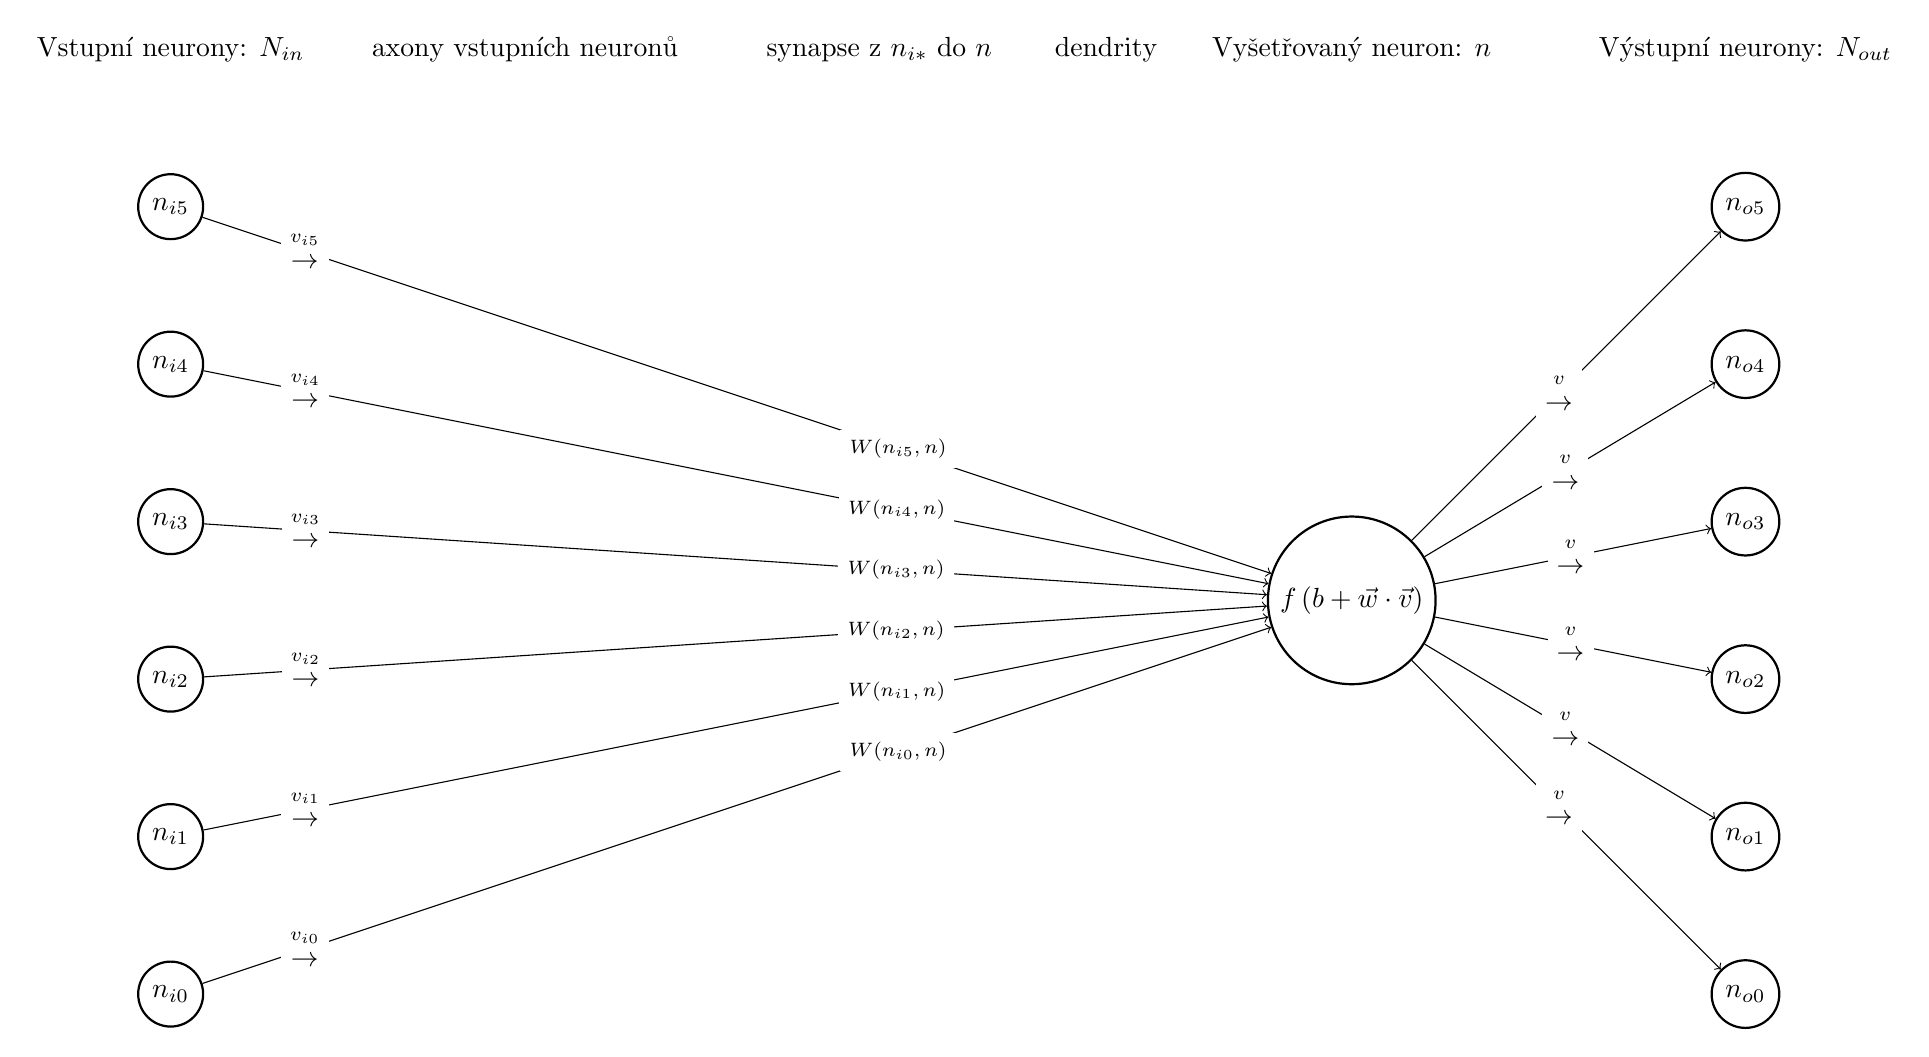
\begin{tikzpicture}
								\def\first{5}
								\def\second{0}
								\def\third{5}
								\node (NI) at (0, 2*\first-3) {Vstupní neurony: $N_{in}$};
								\node (N) at (15, 2*\first-3) {Vyšetřovaný neuron: $n$};
								\node (NO) at (20, 2*\first-3) {Výstupní neurony: $N_{out}$};
								\node (S) at ($(NI)!.60!(N)$) {\Gls{synapse} z~$n_{i*}$ do $n$};
								\node at ($(S)!.48!(N)$) {\Gls{dendrit}y};
								\node at ($(NI)!.5!(S)$) {\Gls{axon}y vstupních neuronů};
																
								\foreach \x in {0,1,...,\first}{%
							    	\node[X] (A\x) at (0, 2*\x-\first) {$n_{i\x}$};
							    }
     
					    	  	\node[X] (B) at (15, -\second) {$f\left(b + \vec{w} \cdot \vec{v} \right)$};
					     
								\foreach \x in {0,1,...,\third}{%
							    	\node[X] (C\x) at (20, 2*\x-\third) {$n_{o\x}$};
							    }
				     
					    		\foreach \x in {0,1,...,\first}{%
						    		\draw [->] (A\x) --node[fill=white, align=center] {\scriptsize $v_{i\x}$\\[-1mm] $\rightarrow$} ($(A\x)!.2!(B)$) -- ($(A\x)!.3!(B)$) -- node[fill=white] {\scriptsize $\W(n_{i\x}, n)$} (B);
							    }
     
				    			\foreach \y in {0,1,...,\third}{%
							    	\draw [->] (B)  -- node[fill=white, align=center] {\scriptsize $v$\\[-1mm] $\rightarrow$} ($(B)!.9!(C\y)$) -- (C\y);
		    					}
						    \end{tikzpicture}
						}
						\caption{Neuron}
						\label{fig:neuron}
					\end{figure}
					
					Označme $\nu = (N,\,W,\,F)$ neuronovou síť, $N$ je množina všech jejích neuronů, $W\!: N\times N \rightarrow \R$ jsou váhy (angl. weights) udávající sílu synapse mezi dvěma neurony (v~případě, že mezi neurony synapse není, je $W$ rovno $0$) a~$F\!: \R^{|N_v|} \rightarrow \R$ je chybová funkce udávající velikost chyby podle rozdílu reálných hodnot od chtěných hodnot výstupních neuronů $\left(N_v\right)$.
			
					Nechť $n \in N, \hspace{1.5ex} n = \left(N_{in},\,N_{out},\,f,\,b,\,v,\,\varepsilon\right)$ je neuron, kde $N_{in} = \left\{n_x \in N|W\left(n_x,\,n\right) \neq 0\right\}$ je množina neuronů, které vysílají signál do $n$, $N_{out} = \left\{n_x \in N|W\left(n,\,n_x\right) \neq 0\right\}$ je množina neuronů, které přijímají signál od $n$, $f\!: \R \rightarrow \R$ je aktivační funkce, $b \in \R$ je bias, $v \in \R$ je signál vycházející z~$n$ a~$\varepsilon$ je chyba (parciální derivace chybové funkce podle $f^{-1}(v)$\footnote{Derivace aktivačních funkcí se často snadno spočítá z~funkční hodnoty, proto uvádím, že hledám derivaci v~bodě, kde je daná funkční hodnota, značím přitom $f^{-1}(y) = x \Leftrightarrow f(x) = y$.}).

				\section{Dopředná propagace}					
					Potom dopředná propagace (tedy spočítání $v$) vypadá takto\footnote{$v_x \in n_x$ značí, že $v_x$ je signál neuronu $n_x$, obdobně u~ostatních informací v~neuronu.}:
					\begin{equation} v~= f\left(b + \sum_{n_x \in N_{in},\,v_x \in n_x} v_x \cdot W\left(n_x,\,n\right) \right) \label{eq:v} \end{equation}
				
					To lze při označení
					\begin{equation} \vec{v} = \left(v_{1},\,v_{2},\,\ldots\right) \label{eq:v2} \end{equation}
					\begin{equation} \vec{w} = \left(w_{1},\,w_{2},\,\ldots\right) \end{equation}
					\begin{equation} \left(\forall n_x \in N_{in}\right)\left(\exists! i~\in \N\right)\left(v_i \in n_x \land w_i = W(n_x, n)\right) \end{equation}
					zapsat vektorově jako:
					\begin{equation} v~= f\left(b + \vec{w} \cdot \vec{v} \right) \label{eq:fp} \end{equation}
				
					Případně můžeme do vektorů \uv{zakomponovat} i~bias\footnote{To v~knihovně není použito z~důvodu netriviálního přidávání prvku do vektoru.}:
					\begin{equation} \vec{v} = \left(1, v_{1},\,v_{2},\,\ldots\right) \end{equation}
					\begin{equation} \vec{w} = \left(b, w_{1},\,w_{2},\,\ldots\right) \end{equation}
					\begin{equation} \left(\forall n_x \in N_{in}\right)\left(\exists! i~\in \N\right)\left(v_i \in n_x \land w_i = W(n_x, n)\right) \end{equation}
					\begin{equation} v~= f\left(\vec{w} \cdot \vec{v} \right) \label{eq:fpb} \end{equation}
					
				\section{Chybová funkce}
					Anglicky loss function nebo někdy také cost function. Udává, nakolik se neuronová síť strefila do správného výstupu. Většinou nás ale nezajímá její hodnota (rozlišujeme pouze, zda síť odpověděla dobře, nebo ne), používáme ji jen jako pomyslné hodnocení ve zpětné propagaci. Její \gls{gradient}, tedy derivace podle všech proměnných (vah a~biasů) v~neuronové síti, totiž udává, jak poupravit hodnoty, aby neuronová síť odpovídala lépe.
				
					Pro naše potřeby stačí pouze jediná chybová funkce
					\begin{equation} E(x) = 0,5\sum_{n_o \in O}\left(v_{od} - v_o\right) \end{equation}
					, kde $O$ je množina výstupních neuronů, $v_o$ jsou jejich výstupní signály a~$v_{od}$ jsou odpovídající chtěné výstupní signály. Tato funkce má výhodu, že její derivace podle libovolného $v_o$ je 
					\begin{equation} \frac{\delta E}{\delta v_o} = v_{od} - v_o \label{eq:ef} \end{equation}
					, tedy $\varepsilon$ výstupních neuronů spočítáme pouze jako rozdíl chtěných a~reálných výstupů.
				
				\section{Zpětná propagace}
					Při zpětné propagaci je důležitý vzorec pro derivaci složené funkce, někdy také znám jako \uv{řetízkové pravidlo} (pro funkci jedné proměnné platí rovnice~(\ref{eq:rp1}), pro více pak rovnice~(\ref{eq:rp2}))\footnote{Pro funkce musí platit, že mají v~daných bodech derivaci, viz \autocite[s. 623]{book:Matanalysis}.}
					\begin{equation} \frac{dy}{dx} = \frac{dz}{dx}\frac{dy}{dz} \label{eq:rp1} \end{equation}
					\begin{equation} \frac{\delta y}{\delta x} = \sum_z\frac{\delta z}{\delta x}\frac{\delta y}{\delta z} \label{eq:rp2} \end{equation}
					Díky tomu můžeme $\varepsilon$ neuronu spočítat pomocí
					\begin{equation} f_x^{-1}(v_x) = \sum_{n_y \in N_{out,\,x},\,v_y \in n_y} v_y \cdot W\left(n_y,\,n_x\right) \label{eq:f1} \end{equation}
					tj.
					\begin{equation} \frac{\delta f_x^{-1}(v_x)}{\delta v_y} = W\left(n_y,\,n_x\right) \end{equation}
					takto:
					\begin{equation} \varepsilon = \frac{ \delta E}{\delta f^{-1}(v)} = \sum_{n_x \in N_{out},\,f_x \in n_x,\,v_x \in n_x}\frac{ \delta E}{\delta f_x^{-1}(v_x)}\cdot\frac{ \delta f_x^{-1}(v_x)}{\delta f^{-1}(v)} \end{equation}
					\begin{equation} \varepsilon = \sum_{n_x \in N_{out},\,f_x \in n_x,\,v_x \in n_x}\frac{ \delta E}{\delta f_x^{-1}(v_x)}\cdot\frac{ \delta f_x^{-1}(v_x)}{\delta v}\cdot\frac{\delta v}{\delta f^{-1}(v)} \end{equation}
					\begin{equation} \varepsilon = \frac{ \delta v}{\delta f^{-1}(v)}\sum_{n_x \in N_{out},\,\varepsilon_x \in n_x}\varepsilon_x \cdot W\left(n,\,n_x\right) \end{equation}
					\begin{equation} \varepsilon = f'\left(f^{-1}(v)\right) \sum_{n_x \in N_{out},\,\varepsilon_x \in n_x} \varepsilon_x \cdot W\left(n,\,n_x\right) \label{eq:bpve} \end{equation}
					
					$\varepsilon$ nás dovede k~tomu, o~kolik musíme posunout bias. Hlavním parametrem neuronové sítě jsou ale váhy (funkce $W$). Derivaci chybové funkce podle váhy určíme za pomoci~rovnice~(\ref{eq:f1}), tj.
					\begin{equation} \frac{\delta f_y^{-1}(v_y)}{\delta W\left(n,\,n_y\right)} = v~\end{equation}
					a~z~rovnice~(\ref{eq:v}):
					\begin{equation} \frac{\delta E}{\delta W\left(n,\,n_y\right)} = \frac{\delta E}{\delta f_y^{-1}\left(v_y\right)}\cdot\frac{\delta f_y^{-1}\left(v_y\right)}{\delta W\left(n,\,n_y\right)} = \varepsilon_y \cdot v~\end{equation}
				
					Obdobně jako v~předchozím případě definujeme vektory\footnote{Značení $\frac{\delta E}{\delta\vec{w}}$ a~$\frac{\delta E}{\delta\W}$ z~rovnic~(\ref{eq:wd}) a~(\ref{eq:wdm}) neznačí derivace podle vektoru a~matice, ale je to symbolické značení pro vektor a~matici derivací podle jednotlivých složek daného tensoru.}:
					
					\begin{equation} \vec{\varepsilon} = \left(\varepsilon_{1},\,\varepsilon_{2},\,\ldots\right) \end{equation}
					\begin{equation} \vec{w} = \left(w_{1},\,w_{2},\,\ldots\right) \end{equation}
					\begin{equation} \frac{\delta E}{\delta\vec{w}} = \left(\frac{\delta E}{\delta w_{1}},\,\frac{\delta E}{\delta w_{2}},\,\ldots\right) \label{eq:wd} \end{equation}
					\begin{equation} \left(\forall n_x \in N_{out}\right)\left(\exists! i~\in \N\right)\left(\varepsilon_i \in n_x \land w_i = W\left(n, n_x\right)\right) \end{equation}
					\begin{equation} \varepsilon = f'\left(f^{-1}(v)\right)\cdot \left(\vec{w} \cdot \vec{\varepsilon}\right) \label{eq:bp1} \end{equation}
					\begin{equation} \frac{\delta E}{\delta\vec{w}} = \vec{\varepsilon}\cdot v~\label{eq:bp2} \end{equation}
					Vektor $\frac{\delta E}{\delta\vec{w}}$ už stačí jen přičíst k~$\vec{w}$, abychom upravili hodnoty $W\left(n, n_x\right)$.
					
					Pomocí tohoto můžeme spočítat všechno kromě $\varepsilon$ na výstupních neuronech. To můžeme z~rovnice~(\ref{eq:ef}) ($n_o \in O$ jsou výstupní neurony, $\varepsilon_o \in n_o$, $f_o \in n_o$ a~$v_o \in n_o$):
					\begin{equation} \varepsilon_o = \frac{\delta E}{\delta f_o^{-1}\left(v_o\right)} = \frac{\delta E}{\delta v_o} \cdot \frac{\delta v_o}{\delta f_o^{-1}\left(v_o\right)} = (v_{od} - v_o) f_o'\left(f_o^{-1}\left(v_o\right)\right) \label{eq:bpout} \end{equation}
					
				\section{Síť} \label{s:n}
					V~sekci~\ref{s:net} jsme se bavili o~tom, že nejpoužívanější sítě mají neurony seřazené do vrstev. Nechť jsou tudíž neurony uspořádány ve vrstvách číslovaných přirozenými čísly od 1 a~nechť jsou navíc i~neurony v~každé vrstvě zvlášť očíslovány přirozenými čísly od 1 (tj.~vrstva je vlastně vektor neuronů). Potom značme $L_x$ vrstvu s~indexem $x$ a~$n_{x,\,y}$ neuron s~indexem $y$ příslušící do $L_x$. To znamená, že pokud $N_{in} \in n_{x,\,y}$, tak $N_{in} = L_{x-1}$, a~pokud $N_{out} \in n_{x,\,y}$, tak $N_{out} = L_{x+1}$. Následně zaveďme vektory ($v_{x,\,i} \in n_{x,\,i}$, $b_{x,\,i} \in n_{x,\,i}$, $f_{x,\,i} \in n_{x,\,i}$ a~$\varepsilon_{x,\,i} \in n_{x,\,i}$):
					
					\begin{equation} \vec{v}_x = \left(v_{x,\,1},\,v_{x,\,2},\,\ldots\right) \end{equation}
					\begin{equation} \vec{w}_{x,\,i} = \left(W\left(n_{x,\,1}, n_{x+1,\,i}\right),\,W\left(n_{x,\,2}, n_{x+1,\,i}\right),\,\ldots\right) \end{equation}
					\begin{equation} \vec{w'}_{x,\,i} = \left(W\left(n_{x,\,i}, n_{x+1,\,1}\right),\,W\left(n_{x,\,i}, n_{x+1,\,2}\right),\,\ldots\right) \end{equation}
					\begin{equation} \vec{b}_x = \left(b_{x,\,1},\,b_{x,\,2},\,\ldots\right) \end{equation}
					\begin{equation} \vec{f}_x = \left(f_{x,\,1},\,f_{x,\,2},\,\ldots\right) \end{equation}
					\begin{equation} \vec{\varepsilon}_x = \left(\varepsilon_{x,\,1},\,\varepsilon_{x,\,2},\,\ldots\right) \end{equation}
					\begin{equation} \frac{\delta E}{\delta\vec{w'}_{x,\,i}} = \left(\frac{\delta E}{\delta W\left(n_{x,\,y}, n_{x+1,\,1}\right)},\,\frac{\delta E}{\delta W\left(n_{x,\,y}, n_{x+1,\,2}\right)},\,\ldots\right) \end{equation}
					
					\subsection{Dopředná propagace}
					Přepíšeme rovnici dopředné propagace~(\ref{eq:fp}):
					\begin{equation} v_{x,\,i} = f_{x,\,i}\left(b_{x,\,i} + \vec{w}_{x-1,\,i} \cdot \vec{v}_{x-1} \right) \end{equation}
					Můžeme využít matici vah a~maticové násobení (aplikaci vektoru funkcí $\vec{f}(\vec{x})$ chápejme tak, že na každou složku $\vec{x}$ se aplikuje odpovídající složka $\vec{f}$):
					\begin{equation}
						\W_x = \begin{pmatrix}
							w_{x,\,1} \\
							w_{x,\,2} \\
							\vdots
						\end{pmatrix} = \begin{pmatrix}
							W\left(n_{x,\,1}, n_{x+1,\,1}\right) & W\left(n_{x,\,2}, n_{x+1,\,1}\right) & \ldots \\
							W\left(n_{x,\,1}, n_{x-1,\,2}\right) & W\left(n_{x,\,2}, n_{x+1,\,2}\right) & \ldots \\
							\vdots & \vdots & \ddots
						\end{pmatrix}
						\label{eq:wm}
					\end{equation}
					\begin{equation} \vec{v}_x = \vec{f}_x\left(\vec{b}_x + W_{x-1} \cdot \vec{v}_{x-1} \right) \label{eq:bpn} \end{equation}
					
					\subsection{Zpětná propagace}
					Nyní přepíšeme rovnice~(\ref{eq:bp1}) a~(\ref{eq:bp2}) zpětné propagace:
					
					\begin{equation} \varepsilon_{x,\,i} = f_{x,\,i}'\left(f_{x,\,i}^{-1}(v_{x,\,i})\right) \odot \left(\vec{w'}_{x,\,i} \cdot \vec{\varepsilon}_{x+1}\right) \label{eq:bp3} \end{equation}
					
					\begin{equation} \frac{\delta E}{\delta\vec{w'}_{x,\,i}} = \vec{\varepsilon}_{x+1}\cdot v_{x,\,i} \label{eq:bp4}\end{equation}
					Rovnici~(\ref{eq:bp3}) můžeme převést hned do maticového tvaru ($\W^T$ značí transponovanou matici $\W$, $\vec{f}^{-1}(x)$ a~$\vec{f}'(x)$ značí aplikaci inverzní funkce a~derivace funkce podobně jako v~(\ref{eq:bpn}), $\odot$~značí násobení po složkách\footnote{Násobením vektorů $\vec{x} = \left(x_1,\,x_2,\,\ldots\right)$ a~$\vec{y} = \left(y_1,\,y_2,\,\ldots\right)$ tzv.~po složkách získáme vektor $\vec{x}\odot\vec{y} = \left(x_1\cdot y_1,\,x_2 \cdot y_2,\,\ldots\right)$.}):
					\begin{equation} \vec{\varepsilon}_x = \vec{f}_x'\left(\vec{f}_x^{-1}(\vec{v}_x)\right) \odot \left(\W_x^T \cdot \vec{\varepsilon}_{x+1}\right)  \label{eq:bpab} \end{equation}
					
					Pro rovnici~(\ref{eq:bp4}) potřebujeme spojit definice~(\ref{eq:wd}) (definice vektoru derivací), kterou přepíšeme do tvaru vrstev:
					\begin{equation} \frac{\delta E}{\delta\vec{w_{x,i}}} = \left(\frac{\delta E}{\delta W\left(n_{x, i}, n_{x+1,1}\right)},\,\frac{\delta E}{\delta W\left(n_{x, i}, n_{x+1,2}\right)},\,\ldots\right) \end{equation}
					a~(\ref{eq:wm}) (definici matice vah):
					\begin{equation}
						\frac{\delta E}{\delta \W_x} = \begin{pmatrix}
							\frac{\delta E}{\delta w_{x,\,1}} \\
							\frac{\delta E}{\delta w_{x,\,2}} \\
							\vdots
						\end{pmatrix} = \begin{pmatrix}
							\frac{\delta E}{\delta W\left(n_{x,\,1}, n_{x+1,\,1}\right)} & \frac{\delta E}{\delta W\left(n_{x,\,1}, n_{x+1,\,2}\right)} & \ldots \\
							\frac{\delta E}{\delta W\left(n_{x,\,2}, n_{x-1,\,1}\right)} & \frac{\delta E}{\delta W\left(n_{x,\,2}, n_{x+1,\,2}\right)} & \ldots \\
							\vdots & \vdots & \ddots
						\end{pmatrix}
						\label{eq:wdm}
					\end{equation}
					
					Nyní jsme již schopni zapsat rovnici~(\ref{eq:bp4}) maticově:
					\begin{equation} \frac{\delta E}{\delta \W_x} = \vec{\varepsilon}_{x+1} \vec{v}_x^T \label{eq:bpab2} \end{equation}

 					I~spočítání $\varepsilon$ u~poslední vrstvy (tj.~neuronů v~$O$, značme ji $L_o$) lze zapsat vektorově ($\vec{v}_{od}$~zde~značí vektor předpokládaných výsledků):
					\begin{equation} \vec{\varepsilon}_o = \vec{f}_x'\left(\vec{f}_x^{-1}(\vec{v}_x)\right) \odot \left(\vec{v}_{od} - \vec{v}_o\right) \label{eq:bpab3} \end{equation}
					
					\subsection{Zakomponování biasu}
					Nejdříve musíme upravit vektory a~matice:
					\begin{equation} \vec{v}_x = \left(1,\,v_{x,\,1},\,v_{x,\,2},\,\ldots\right) \end{equation}
					\begin{equation} \vec{f}_x = \left(1,\,f_{x,\,1},\,f_{x,\,2},\,\ldots\right) \end{equation}
					\begin{equation} \vec{\varepsilon}_x = \left(0,\,\varepsilon_{x,\,1},\,\varepsilon_{x,\,2},\,\ldots\right) \end{equation}
					\begin{equation}
						\W_x = \begin{pmatrix}
							1 & 0 & 0 & \ldots \\
							b_{x+1,\,1} & W\left(n_{x,\,1}, n_{x+1,\,1}\right) & W\left(n_{x,\,2}, n_{x+1,\,1}\right) & \ldots \\
							b_{x+1,\,2} & W\left(n_{x,\,1}, n_{x-1,\,2}\right) & W\left(n_{x,\,2}, n_{x+1,\,2}\right) & \ldots \\
							\vdots & \vdots & \vdots & \ddots
						\end{pmatrix}
					\end{equation}
					\begin{equation}
						\frac{\delta E}{\delta \W_x} = \begin{pmatrix}
							0 & 0 & 0 & \ldots \\
							\frac{\delta E}{\delta b_{x+1,\,1}} & \frac{\delta E}{\delta W\left(n_{x,\,1}, n_{x+1,\,1}\right)} & \frac{\delta E}{\delta W\left(n_{x,\,1}, n_{x+1,\,2}\right)} & \ldots \\
							\frac{\delta E}{\delta b_{x+1,\,2}} & \frac{\delta E}{\delta W\left(n_{x,\,2}, n_{x-1,\,1}\right)} & \frac{\delta E}{\delta W\left(n_{x,\,2}, n_{x+1,\,2}\right)} & \ldots \\
							\vdots & \vdots & \vdots & \ddots
						\end{pmatrix}
					\end{equation}
					
					Rovnice~(\ref{eq:bpn}) (samozřejmě bez biasu:
					\begin{equation} \vec{v}_x = \vec{f}_x\left(W_{x-1} \cdot \vec{v}_{x-1} \right) \label{eq:bpnb} \end{equation}
					),~(\ref{eq:bpab}) a~(\ref{eq:bpab2}) poté fungují pořád stejně. Rovnice~(\ref{eq:bpab3}) funguje také shodně, jelikož prostě řekneme, že první člen odhadu vyšel tak, jak má, tj.~$\vec{\varepsilon} = \left(0,\,\ldots\right)$
				
				\section{Aktivační funkce} \label{s:af}
					Jelikož neurony mají bias, není nutné udávat aktivační funkce obecně, stačí je jen udat tak, že $x=0$ odpovídá mezi v~pomyslném biologickém neuronu. Mezi aktivační funkce\footnote{Funkce jsem čerpal převážně z~\autocite{wiki:ActivationFunctions}.} patří:
					\begin{itemize}
						\item \emph{Binary step}
							\begin{equation}f(x) = \begin{cases}0, & \text{když } x < 0\\1, & \text{když } x \geq 0 \end{cases}\end{equation}
							\begin{equation}f'(x) = \begin{cases}0, & \text{když } x \neq 0\\\mathrm{+\infty}, & \text{když } x = 0 \end{cases}\end{equation}
							(česky \emph{binární krok}), již zmíněná funkce, jež odpovídá reálnému neuronu, ale není použitelná pro učení na základě \gls{gradient}u, jelikož má derivaci 0 všude kromě bodu $x = 0$, kde je nespojitá.
						
					    	\figF{binaryStep}{Binární krok}
						
						\item \emph{Identity}
							\begin{equation}f(x) = x\end{equation}
							\begin{equation}f'(x) = 1 \end{equation}
							(česky \emph{identita}) odpovídá stavu, jako kdyby tam žádná funkce nebyla. Její derivace je 1, tedy se velmi snadno určí v~libovolném bodě.	
											
						    \figF{identity}{Identita}
					    
						\item \emph{Sigmoid} \autocite{article:AF} (značí se $\sigma$)
							\begin{equation}\sigma(x) = \frac{1}{1+e^{-x}}\end{equation}										
							\begin{equation}\sigma'(x) = \frac{e^{-x}}{\left(1+e^{-x}\right)^2} = \frac{1}{1+e^{-x}}\left(1-\frac{1}{1+e^{-x}}\right) = \sigma(x)\cdot\left(1-\sigma(x)\right)\end{equation}										
							je jedna z~nejznámějších aktivačních funkcí. Je to vlastně takový hladký přechod mezi 0 a~1. Také je na $\sigma$ dobře vidět, proč se často počítá derivace z~funkční hodnoty, místo počítání exponenciální funkce a~dělení si vystačíme s~násobením a~odčítáním. \emph{Sigmoida} se také používá ve spojení s~ostatními funkcemi, většinou $\sigma(x)$ pro kladné a~druhá funkce pro záporné.
						
					   		\figF{sigmoid}{$\sigma$}
							
						\item Nesmíme zapomenout na \emph{sigmoidě} podobnou a~také často používanou funkci \emph{hyperbolický tangens} ($\tanh$) \autocite{article:AF} \autocite{book:FFActivationFunctions}:
							\begin{equation}\tanh(x) = \frac{\sinh(x)}{\cosh(x)} = \frac{e^x-e^{-x}}{e^x+e^{-x}} = \frac{2}{1-e^{-2x}} - 1 = 2\cdot\sigma(2x)-1\end{equation}										
							\begin{equation}\tanh'(x) = \frac{1}{\cosh^2(x)} = \frac{\cosh^2(x) - \sinh^2(x)}{\cosh^2(x)} = 1-\tanh^2(x)\end{equation}		
							\begin{equation}\tanh'(x) = 4\cdot \sigma'(2x) = 4\cdot\sigma(2x)\cdot\left(1 - \sigma(2x)\right)\end{equation}
							Největší rozdíl oproti $\sigma$ je, že může nabývat i~záporných hodnot, což sice moc neodpovídá přírodnímu neuronu, ale když si rozmyslíme, že stačí zvětšit biasy u~neuronů, do kterých neuron s~aktivační funkcí $\tanh$ vysílá signál, dospějeme k~výsledku, že tato funkce také funguje.
						
				    		\figF{tanh}{Hyperbolický tangens}
						
						\item Další funkce s~vazbou na \emph{sigmoidu} je funkce \emph{swish} \autocite{article:AF}:
							\begin{equation}f(x) = x\cdot \sigma(x) = \frac{x}{1+e^{-x}}\end{equation}		
							\begin{equation}f'(x) = x + \sigma'(x) = x + \sigma(x)\cdot\left(1-\sigma(x)\right) \end{equation}					
							Nepodařilo se mi ale najít derivaci za pomoci funkční hodnoty.
							
					    	\figF{swish}{Swish}
						
						
						\item Ukazuje se, že identita jako taková se v~podstatě použít nedá, ale hojně využívaná je její \uv{upravená} verze \emph{rectified linear unit} \autocite{article:AF} (česky něco jako \emph{napravená přímá úměrnost}), která záporná čísla převádí na nulu a~v~kladných se chová jako \emph{identita}:
							\begin{equation}f(x) = \begin{cases}0, & \text{když } x < 0\\x, & \text{když } x \geq 0 \end{cases}\end{equation}
							\begin{equation}f'(x) = \begin{cases}0, & \text{když } x < 0\\1, & \text{když } x > 0 \\\text{neexistuje}, & \text{když } x = 0 \end{cases}\end{equation}
							Trochu připomíná biologický neuron, protože pro záporné hodnoty nevysílá, ale na rozdíl od něj má variabilní hodnotu vysílaného signálu. Často se například používá ve filtrech, jelikož chceme detekovat, zda je někde hrana, ale nechceme vysílat záporný signál, když někde hrana není, protože může být o~pixel vedle. 
							
						    \figF{rectifiedLinearUnit}{Rectified linear unit}
						
						\item Kromě této verze je v~knihovně ještě \emph{leaky} (děravá či prosakující) \emph{rectified linear unit} \autocite{article:AF}, která v~záporných hodnotách nedává nulu, ale \emph{přímou úměrnost}.
					
						    \figF{hardHyperbolicFunction}{Hard hyperbolic function}
						    
						\item K~těmto funkcím můžeme přiřadit i~\emph{hard hyperbolic function}, která je \emph{identitou} pouze na intervalu $(-1, 1)$, tedy odpovídá biologickému neuronu asi nejvíce z~těchto \uv{lineárních funkcí}.
												    
							\figF{leakyRectifiedLinearUnit}{Leaky rectified linear unit pro koeficient úměrnosti 0.1}

						
						
						\item \emph{Rectified unit} není hladká (nemá derivaci v~bodě nula), ale to lze napravit, když použijeme funkci \emph{soft plus} \autocite{article:AF} ($\ln\left(1+e^x\right)$). Podobnou úpravu lze udělat i~s~funkcí \emph{signum} (\emph{znaménko}, často se značí \emph{sign}), což je téměř \emph{binární krok}\footnote{Z důvodu téhle podobnosti není ani implementována.}, akorát v~záporných hodnotách nabývá funkční hodnoty -1 místo 0. \emph{Signum} se dá zapsat jako podíl $x$ a~$|x|$, tudíž tato úprava (\emph{soft sign} \autocite{article:AF}) vypadá následovně:
							\begin{equation} f(x) = \frac{x}{|x| + 1} \end{equation}
											
							\begin{figure}[h]
							    \centering
							    \figSF{softPlus}{Soft plus}
						    	\figSF{softSign}{Soft signum}
						    	\caption{Soft funkce}
							\end{figure}
						
						\item Jednou skupinou funkcí, se kterými se sice experimentuje, ale stěží najdete nějaké využití, jsou ty, které nejsou monotonní\footnote{Můžeme si všimnout, že téměř všechny předchozí funkce jsou neklesající, většina dokonce rostoucí na celém definičním oboru.}, jako sinus, kosinus, \emph{Gaussova funkce} ($e^{-x^2}$), apod. Vzhledem k~jejich mizivému využití je implementován pouze \emph{sinus}.
						
							\figF{sin}{Sinus}
							
					\end{itemize}
			
				\section{Shrnutí}
					Rovnice:
					\begin{itemize}
						\item Dopředné propagace, tj.~(\ref{eq:fp}) resp.~(\ref{eq:fpb}) nebo~(\ref{eq:bpn}) resp.~(\ref{eq:bpnb}):
							$$ v~= f\left(b + \vec{w} \cdot \vec{v} \right) $$
							$$ v~= f\left(\vec{w} \cdot \vec{v} \right) $$
							$$ \vec{v}_x = \vec{f}_x\left(\vec{b}_x + W_{x-1} \cdot \vec{v}_{x-1} \right) $$
							$$ \vec{v}_x = \vec{f}_x\left(W_{x-1} \cdot \vec{v}_{x-1} \right) $$
						\item Zpětné propagace, tj.~(\ref{eq:bpve}) a~(\ref{eq:bp2}) nebo~(\ref{eq:bpab}) a~(\ref{eq:bpab2}):
							$$ \varepsilon = f'\left(f^{-1}(v)\right) \sum_{n_x \in N_{out},\,\varepsilon_x \in n_x} \varepsilon_x \cdot W\left(n,\,n_x\right) $$
							$$ \frac{\delta E}{\delta\vec{w}} = \vec{\varepsilon}\cdot v~$$
							$$ \vec{\varepsilon}_x = \vec{f}_x'\left(\vec{f}_x^{-1}(\vec{v}_x)\right) \odot \left(\W_x^T \cdot \vec{\varepsilon}_{x+1}\right) $$
							$$ \frac{\delta E}{\delta \W_x} = \vec{\varepsilon}_{x+1} \vec{v}_x^T $$
						\item Prvotní části zpětné propagace, tj.~(\ref{eq:bpout}) nebo~(\ref{eq:bpab3})
							$$ \varepsilon_o = (v_{od} - v_o) f_o'\left(f_o^{-1}\left(v_o\right)\right) $$
							$$ \vec{\varepsilon}_o = \vec{f}_x'\left(\vec{f}_x^{-1}(\vec{v}_x)\right) \odot \left(\vec{v}_{od} - \vec{v}_o\right) $$
					\end{itemize}
					nám popisují matematiku stojící za fungováním neuronových sítí, tedy naším cílem bude je implementovat. Navíc k~implementování těchto rovnic potřebujeme naprogramovat samotný neuron, který jsme si definovali v~sekci~\ref{s:neuron} jako:
						$$ n = \left(N_{in},\,N_{out},\,f,\,b,\,v,\,\varepsilon\right) $$
					Také často používáme aktivační funkce, proto by v~naší knihovně neměly chybět.
		
	\part{Praktická část}
			\noindent Cílem této práce je knihovna, která nám umožní používat neuronové sítě v~\gls{Kotlin}u. Jak bylo řečeno na konci minulé kapitoly, musí obsahovat aktivační funkce, nejlépe všechny uvedené v~sekci~\ref{s:af}, zároveň však umožnit uživateli definovat si funkce vlastní. Poté se zaměříme hlavně na neuronovou síť obsahující vrstvy, její implementace bude zároveň zahrnovat jak implementaci neuronu, tak implementaci dopředné a~zpětné propagace.
			
			Konvoluční síť pro jednoduchost naprogramujeme za použití sítí s~vrstvami, tedy jedinou věc, kterou potřebujeme implementovat, je způsob používání filtru. Nakonec se podíváme i~na asociativní paměť, pro kterou navíc potřebujeme naprogramovat neurony, jelikož na rozdíl od neuronové sítě s~vrstvami zde nelze ukládat jednotlivé hodnoty neuronu pohromadě (např.~všechny $v$ do jednoho pole, nebo všechny $\varepsilon$ do jiného).
		
			Aby nemuselo být v~knihovně implementováno maticové násobení, použil jsem knihovnu \verb!koma! (celým názvem Kotlin math), která implementuje základy lineární algebry v~\gls{Kotlin}u. Knihovna je pro \gls{JVM}, Javascript i~pro binární kód, avšak ve Windows ji nelze zkompilovat, proto naše knihovna funguje pouze pro \gls{JVM} a~Javascript. \autocite{online:Koma}
			
			\noindent\hrulefill
			
			Asociativní paměť se mi bohužel nepodařilo doprogramovat do konce, natož otestovat, tedy není uvedena dále v~této kapitole. Implementaci neuronu nalezneme v~\verb!core! (viz níže) jako \glsdisp{trida}{třídu} \verb!Neuron!, která se stará přímo o~výpočty z kapitoly~\ref{s:fn}. Uchovávání těchto neuronů a~spouštění výpočtů na každém z~nich má na starosti \gls{trida} \verb!AssociativeMemory! taktéž z~\verb!core!.
	
		\chapter{Struktura knihovny}
		
			\begin{figure}
				\begin{forest}
					for tree={
					  draw,
					  minimum width=3.1cm,
					  anchor=west,
					  align=center,
					  child anchor=west,
					  grow'=east,
					},
					[{\texttt{NeuralNetwork}}
						[{\texttt{core}}, name=p
						  	[{\texttt{IActivation}\\\texttt{Functions}}, name=i
								[{\texttt{ActivationFunctions}}, name=c]
								[{\texttt{CustomFunction}}]
						  	]
							[{\texttt{INeural}\\\texttt{Network}}
								[{\texttt{BasicNeuralNetwork}}]
								[{\texttt{ConvolutionalNeural}\\\texttt{Network}}]
								[{\texttt{AssociativeMemory}}]
							]
						]
						[{\texttt{mnistdatabase}}
							[{\texttt{TrainingData}}
								[\texttt{MnistTrainingData}]
							]
						]
					]
					\node[anchor=south,align=center] 
					  at ([yshift=1cm]p|-c) {balíčky};
					\node[anchor=south,align=left] 
					  at ([yshift=1cm]i|-c) {\gls{rozhrani}};
					\node[anchor=south,align=left] 
					  at ([yshift=1cm]c|-c) {\glsdisp{trida}{třídy}, \gls{enum}s};
				\end{forest}
				\caption{Struktura knihovny}
			\end{figure}
			
			
			
			Knihovna je rozdělena do dvou \glsdisp{balicek}{balíčků}:
			\begin{itemize}
				\item První, a~ten hlavní, je \verb!core! (česky jádro), které obsahuje definice neuronových sítí (tj.~konvoluční neuronovou síť, obyčejnou neuronovou síť, asociativní paměť) a~definice pro ně potřebné (například aktivační funkce). Právě v~tomto \glsdisp{balicek}{balíčku} je implementováno to, co bylo v~teoretické části.
				\item Druhý je \verb!mnistDatabase!, která se stará o~učení neuronových sítí na datech z~databází ve formátu MNIST. O~databázích ve formátu MNIST se v~teorii nepsalo, jsou zmíněny až přímo v~sekci~\ref{sec:md}, která pojednává o~tomto balíčku.
			\end{itemize}
			
			\section{\texttt{core}}
			
				\subsection{\texttt{IActivationFunctions}}
					\Gls{rozhrani}, které zahrnuje \verb!ActivationFunction! a~\verb!CustomFunction!. Jeho instance se používají jako aktivační funkce. Funkce lze zavolat s~parametrem \gls{typ}u \verb!Double!, což nám dá hodnotu funkce v~tomto bodě, popřípadě lze obdobně zavolat jejich dvě metody \verb!xD! a~\verb!yD! udávající v~pořadí hodnotu derivace v~bodě x a~v~bodě, kde je funkční hodnota rovna parametru.
			
				\subsection{\texttt{ActivationFunctions}}
					\Gls{enum} častých funkcí, jež se používají jako aktivační funkce v~neuronech. Některé jsou označeny jako překonané (anglicky deprecated), jelikož u~funkcí, které nejsou všude hladké, neexistuje všude derivace. Taktéž u~funkcí, jež nejsou prosté, nelze vždy určit derivaci podle funkční hodnoty.
					
					Implementovány jsou všechny funkce uvedené v~sekci~\ref{s:af}
					
				\subsection{\texttt{CustomFunction}}
					Poskytuje možnost implementovat si vlastní aktivační funkci, má stejné metody (zde jsou to vlastnosti \gls{typ}u \verb!() -> Unit!) jako ActivationFunctions.
			
				\subsection{\texttt{INeuralNetwork}}
					\Gls{rozhrani}, které implementuje základní funkce neuronových sítí, které mají jako vstup i~výstup vektor \verb!Double!. Obsahuje funkce:
					\begin{itemize}
						\item \verb!run(vstupní vektor)!, která je koncipována tak, aby ze vstupního vektoru spočítala vektor výstupní (tedy většinou udělala dopřednou propagaci). Jako vstupní vektor lze dát jak \glsref{Double}\verb!Matrix<Double>! z~knihovny \verb!koma!, tak \glsref{DoubleArray}\verb!DoubleArray!, které je převedeno na \glsref{Double}\verb!Matrix<Double>!, následně se zavolá funkce \verb!run! s~tímto \gls{typ}em a~výstup se převede zpět na \glsref{DoubleArray}\verb!DoubleArray!.\footnote{\glsref{DoubleArray}\verb!DoubleArray! je použito, protože je to \gls{typ} \gls{Kotlin}u samotného, ale jelikož matematika v~neuronových sítích je implementována pomocí \glsref{Double}\verb!Matrix<Double>!, musí se převést mezi \gls{typ}y.}
						
						Navíc (hlavně kvůli konvolučním neuronovým sítím) může být vstup i~dvourozměrný, v~tomto případě je pak nutno u~\glsref{DoubleArray}\verb!DoubleArray! uvést i~šířku řádku.
						\item \verb!train(vstupní vektor, chtěný výstupní vektor)! resp. \verb!train(vstupní vektory, chtěné výstupní vektory)!, která je koncipována tak, aby nejdříve provedla \verb!run(vstupní vektor)!, výsledek porovnala s~chtěným a~přepočítala váhy v~neuronové síti tak, aby se výstup \verb!run(vstupní vektor)! přiblížil (zmenšila se velikost jejich rozdílu) chtěnému výstupnímu vektoru. Kromě verze s~parametry \gls{typ}u \glsref{DoubleArray}\verb!DoubleArray! je funkce implementována i~pro \gls{typ} \glsref{Array}\glsref{DoubleArray}\verb!Array<DoubleArray>!, tedy trénovací vstupy a~výstupy lze vložit i~všechny najednou.
					\end{itemize}
			
				\subsection{\texttt{BasicNeuralNetwork}}
					Tato \gls{trida} \gls{rozhrani} INeuralNetwork implementuje nejčastěji používanou neuronovou síť, kde jsou neurony uspořádány do vrstev a~ovlivňují se pouze jedním směrem. Parametry, které lze nastavit, jsou:
					\begin{itemize}
						\item \verb!numberOfHiddenLayers!, neboli počet skrytých vrstev (tj.~ty, jež jsou mezi vstupní a~výstupní vrstvou). Čím více vrstev je nastaveno, tím hůře se síť učí, většinou je proto třeba nastavit pouze jednu skrytou vrstvu nebo nastavit velmi malou hodnotu \verb!learning rate! (proměnná, jež není v~konstruktoru, která udává rychlost změn vah).
						\item \verb!activationFunctions!, česky aktivační funkce, musí být vybrána z~\glsdisp{trida}{třídy} ActivationFunction. Při použití funkcí, které nejsou hladké, se neurony mohou chovat nepředvídatelným způsobem.
					\end{itemize}
					
				\subsection{\texttt{ConvolutionalNetwork}}
					Tato \gls{trida} \gls{rozhrani} INeuralNetwork implementuje konvoluční neuronové sítě. Její konstruktor přijímá dva parametry \gls{typ}u \verb!BasicNeuralNetwork!, první je filtr, druhá je samotná neuronová síť. Dalším parametrem je logická hodnota, zda se má i~filtr učit (to se ale téměř nepoužívá, takže je tato hodnota při neuvedení nastavena na \glsref{false}\verb!false!).
					
					\Gls{cobject} této \glsdisp{trida}{třídy} navíc obsahuje příklad takového filtru (jednoduchý filtr detekující hrany viz obrázek~\ref{fig:filter})
					\begin{figure}
						\resizebox{\textwidth}{!}{%
							\begin{tikzpicture}
					    		\foreach \x in {-1,0,1}{%
						    		\foreach \y in {-1,0,1}{%
										\node[S] (NI) at (\x, \y) {$\y$};
									}
								}
					    		\foreach \x in {-1,0,1}{%
						    		\foreach \y in {-1,0,1}{%
										\node[S] (NI) at (5+\x, -\y) {$\y$};
									}
								}
					    		\foreach \x in {-1,0,1}{%
						    		\foreach \y in {-1,0,1}{%
										\node[S] (NI) at (10+\y, \x) {$\y$};
									}
								}
					    		\foreach \x in {-1,0,1}{%
						    		\foreach \y in {-1,0,1}{%
										\node[S] (NI) at (15-\y, \x) {$\y$};
									}
								}
								
								
					    		\foreach \x in {-1,0,1}{%
						    		\foreach \y in {-1,0,1}{%
										\node[S] (NI) at (\y, 5+\x) {$\pgfmathparse{(\x+\y)/abs(\x+\y)}\pgfmathprintnumber[fixed,fixed zerofill,precision=0]\pgfmathresult$};
									}
								}\foreach \x in {-1,0,1}{%
						    		\foreach \y in {-1,0,1}{%
										\node[S] (NI) at (5-\y, 5+\x) {$\pgfmathparse{(\x+\y)/abs(\x+\y)}\pgfmathprintnumber[fixed,fixed zerofill,precision=0]\pgfmathresult$};
									}
								}\foreach \x in {-1,0,1}{%
						    		\foreach \y in {-1,0,1}{%
										\node[S] (NI) at (10-\y, 5-\x) {$\pgfmathparse{(\x+\y)/abs(\x+\y)}\pgfmathprintnumber[fixed,fixed zerofill,precision=0]\pgfmathresult$};
									}
								}\foreach \x in {-1,0,1}{%
						    		\foreach \y in {-1,0,1}{%
										\node[S] (NI) at (15+\y, 5-\x) {$\pgfmathparse{(\x+\y)/abs(\x+\y)}\pgfmathprintnumber[fixed,fixed zerofill,precision=0]\pgfmathresult$};
									}
								}
						    \end{tikzpicture}
						}
						\caption{Ilustrace filtru z~\glsdisp{trida}{třídy} ConvolutionalNetwork, vstupem je matice $3\times 3$ pixely, ta se po složkách násobí vždy s~1 z~8 matic výše, sečtou se všechny prvky výsledné matice, aplikuje se \emph{rectified linear unit} a~každé z~výsledných 8 čísel pak udává, jak moc je v~původní matici hrana odpovídající dané matici výše (tzn.~jak moc je pixel násobený 1 bílý a~pixel násobený -1 černý)}
						\label{fig:filter}
					\end{figure}
			
			\section{\texttt{mnistDatabase}} \label{sec:md}
				Pro otestování knihovny je potřeba nějaký dataset. K~tomuto účelu je v~knihovně implementována \gls{trida} \verb!TrainingDataMnist!, která umí přečíst data z~databáze MNIST a~EMNIST. Poté poskytuje vždy jedno zadání (obrázek číslice / písmena) a~jeho řešení (ve formě vektoru, kde pouze na správném místě je 1, jinak je všude 0).
				
				Jako parametry přijímá řetězec (\verb!String!) s~názvem souboru s~obrázky a~řetězec s~názvem souboru s~daty (identifikací toho, co je na obrázcích). Zároveň nastavením parametru \verb!inverse! na \glsref{true}\verb!true! lze převrátit osy obrázku (viz~obrázek~\ref{EMNIST}). Tato \gls{trida} zatím funguje pouze v~\gls{JVM}, jelikož používá funkci na načtení souboru a~tuto funkci jsem zatím v~Javascriptu neimplementoval (soubor je většinou uložen někde na serveru, takže je obtížnější ho načíst).
				
				Dále tento \gls{balicek} rozšiřuje rozhraní \verb!INeuralNetwork! o~funkci \verb!train! s~parametrem \gls{typ}u \verb!TrainData!, což je pouze \verb!typealias! (tzn.~jiný název pro \gls{typ} v~\gls{Kotlin}u) za \glsref{DoubleArray}\glsref{Pair}\verb!Sequence<Pair<DoubleArray, DoubleArray>>!, jež je implementován výše zmíněnou \glsdisp{trida}{třídou} \verb!TrainingDataMnist!.
				
				\subsection{Databáze MNIST}
					\uv{Databáze MNIST, dataset ručně psaných číslic dostupná na stránkách \url{http://yann.lecun.com/exdb/mnist/} obsahuje 60\,000 tréninkových a~10\,000 ověřovacích příkladů. MNIST vychází z~databáze spravované NIST (National Institute of Standarts and Technology). Číslice mají normalizovanou velikost a~jsou vycentrované v~obrázcích shodné velikosti.} \parencite[přeloženo]{online:MNIST} Ukázku takových obrázků vidíme na obrázku~\ref{fig:MNIST}.
					
					\begin{figure}
						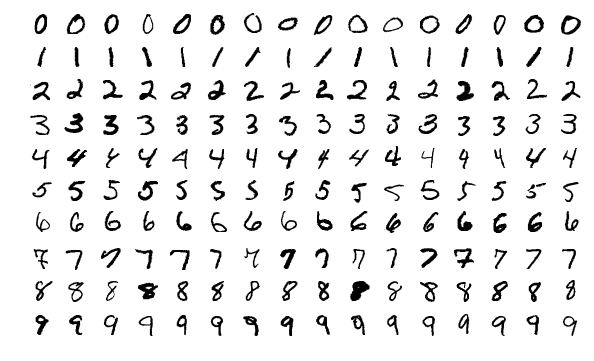
\includegraphics[width=0.95\linewidth]{MnistExamples.png}
						\caption{Příklad obrázků z~databáze MNIST \autocite{wiki:MNIST}}
						\label{fig:MNIST}
					\end{figure}
					
					Tuto databázi jsem použil pro první testování své \verb!BasicNeuralNetwork!, jelikož má pro první testování dostačující velikost. Pro pozdější testování využívám převážně EMNIST.
				\subsection{Databáze EMNIST} \label{EMNIST}
					\uv{Databáze MNIST se stala standardem pro učení umělého vidění. Databáze MNIST je odvozená z~databáze NIST Special Database 19, která obsahuje ručně psané číslice a~velká i~malá písmena. EMNIST (Extended MNIST), varianta celé databáze NIST, přebírá uspořádání z~databáze MNIST\footnote{Má však prohozené řádky a~sloupce pixelů v~obrázcích.}.} \parencite[přeloženo]{article:EMNIST}
					
					Tato databáze obsahuje více příkladů než MNIST, navíc obsahuje i~sety s~písmeny, proto jsem po prvních pokusech s~MNIST přešel na tuto databázi.

		\chapter{Používání knihovny}
			\section{Trénování sítě}
				Příklad takového tréninku je v~souboru \verb!NeuralNetworkTestJVM! funkce \verb!mnist()!. Takové trénování ale trvá více než deset minut (konkrétně tato funkce běží asi tři čtvrtě hodiny), tudíž ho nelze zahrnout do testů. V~testech je pouze trénování malinké sítě, aby fungovala jako \gls{xor}.
			
				Nejprve musíme neuronovou síť natrénovat a~uložit. Trénování neuronové sítě probíhá za pomoci funkce \verb!train!. Té musíme poskytovat tréninkové vstupy s~odpovídajícími výstupy, což můžeme udělat tak, že funkci \verb!train! budeme volat z~\glsdisp{cyklus}{cyklu}, který bude tato data postupně načítat. Dalším způsobem je předat rovnou celý \glsref{Array}\verb!Array! vstupů a~výstupů, to ale často znamená načíst miliony objektů \glsdisp{trida}{třídy} \glsref{Double}\verb!Double!, proto to může výrazně zpomalit učení. Poslední možností (pokud máme data ve formátu MNIST) je využít \glsdisp{trida}{třídy} \verb!TrainingData!, které poskytneme soubory s~daty a~ona vytvoří příslušné objekty \gls{typ}u \glsref{Double}\verb!Double! až ve chvíli, kdy dojde na danou dvojici vstup -- výstup.
				
				Dobré je také během učení pomalu snižovat \verb!learningRate!, jelikož nejdřív se neuronová síť vlastně učí hlavně konkrétní obrázky (v~této fázi nejlépe poznává obrázky, které dostala v~tréninku naposledy), poté ale umí čím dál více věcí a~nechceme, aby se přepisovaly již nabyté vědomosti. Já jsem například trénoval síť desetkrát na stejných datech (to není úplně vhodné, data by se měla měnit, aby se co nejméně naučila konkrétní obrázky\footnote{Při opakování malého datasetu se může stát, že neuronová síť bude umět rozpoznat jen obrázek, který je na pixel přesně shodný s~tréninkovými obrázky.}, ale pro jednoduchost to stačí) s~tím, že pokaždé jsem \verb!learningRate! vydělil 1,5.
				
				Poté už můžeme síť hned používat (například ji otestovat), ale většinou ji chceme používat víckrát a~třeba i~v~rámci jiného programu. Proto mají \glsdisp{trida}{třídy} \gls{rozhrani} \verb!INeuralNetwork! funkci \verb!save!, která vrátí data neuronové sítě jako řetězec (takový \uv{osekaný} \gls{JSON}), který je pak možno uložit. V~\gls{JVM} je přímo definována funkce \verb!saveFile(název souboru, data)!.
				
			\section{Používání sítě}
				Ukázka načítání sítě je v~programu \verb!JSTest2! řádek 43 až 45 a~ukázka výpočtu je parametr funkce \verb!evaluateButton.addEventListener!. Můžete si všimnout, že použití je v~rámci jednotek řádků kódu, zbytek se pouze stará o~uživatelský vstup (program funguje jak za pomoci klikání myší, tak v~mobilu pomocí dotyku).
				
				Jakmile máme nějakou síť natrénovanou a~uloženou v~řetězci, můžeme ji znovu nahrát pomocí funkce \verb!load(data)! nacházející se v~\gls{cobject}u \glsdisp{trida}{třídy} \verb!BasicNeuralNetwork! nebo \verb!ConvolutionalNeuralNetwork!. Návratovou hodnotou této funkce je samotná neuronová síť, takže ji stačí uložit do proměnné, na které pak zavoláme funkci \verb!run! s~vstupním vektorem jako parametrem a~tím získáme výstupní vektor, který stačí už jen zpracovat (např. při rozpoznávání číslic to znamená zjistit, který z~výsledných 10 neuronů vysílá největší výstupní signál).
				
		
			\section{Nastavení hodnot}
				Neuronová síť má mnoho hodnot, které lze nastavit. Knihovna je vyzkoušena na rozpoznávání čísel v~databázích MNIST a~EMNIST s následujícím nastavením hodnot:
				\begin{itemize}
					\item Learning rate na 0.1 a každou z 10 epoch (1 epocha = 1 průchod přes všechny obrázky) se snižuje na $\frac{2}{3}$ původní hodnoty.
					\item Počet skrytých vrstev na jedna (dvě už se nenaučí propojit vstup s~výstupem a~bez skryté vrstvy síť vůbec nefunguje\footnote{Pokud byste potřebovali učit síť s~více skrytými vrstvami, musíte nastavit learning rate na daleko nižší hodnotu a učit síť daleko déle a na více vstupech.}).
					\item Počet neuronů ve skryté vrstvě na 100 (snížení počtu neuronů výsledky zhorší, zvýšení na 200 až 300 výsledky moc nezlepší, navíc trénování větší sítě zabere mnohem více času).
					\item Aktivační funkce na sigmoidu (jiné jsem moc nezkoušel, sigmoida stačí).
				\end{itemize}


	\appendix
	\addcontentsline{toc}{part}{Apendix}
	
	\chapter*{Závěr}
	
		Cílem mé práce bylo implementovat neuronovou síť, což se mi podařilo dokonce do takové míry, že v~programu, kde zabírá pár řádků, je schopna rozeznávat číslice (ukázka je na stránkách \url{moznabude.cz}, nebo na přiloženém USB). Největším přínosem je asi \gls{trida} \verb!BasicNeuralNetwork!, která implementuje velkou část matematiky obtížnou na rozmyšlení a~stojící za téměř všemi neuronovými sítěmi, o~niž se programátor v~\gls{Kotlin}u díky mojí knihovně už nemusí starat.
		
		Zároveň jsem si díky rozdělení do balíčků a~využití možností objektově orientovaného programování připravil dobrý podklad pro rozšiřování knihovny. Dále bych mohl pokračovat například implementováním lepšího ukládání do souboru (ukládání \gls{typ}u \glsref{Double}\verb!Double! jako textového řetězce není moc efektivní), implementování některých genetických algoritmů, či naprogramování konvoluční sítě tak, aby filtry mohly pracovat $n$ rozměrně.
		
		Pro mě samotného byl asi největší přínos, že jsem si poprvé zkusil napsat formálnější kód a~to jak v~\gls{Kotlin}u, tak i~v~LaTeXu. Navíc, už jen rozmyšlení si, co má tento text obsahovat byla pro mě velká životní zkušenost.
	
	\nocite{*}
    \printglossary[title={Slovníček pojmů}]	% Vytvoří seznam zkratek
    \printbibliography					% Vytvoří seznam literatury
	\addcontentsline{toc}{chapter}{Bibliografie}
    \listoffigures						% Vytvoří seznam obrázků
	\addcontentsline{toc}{chapter}{Seznam obrázků}
    %\listoftables						% Vytvoří seznam tabulek
    
    \begin{prilohy}
    	\eitem{Zdrojový kód knihovny} (složka NeuralNetwork)
    	\eitem{Dokumentace} (složka Dokumentace)
    	\eitem{Testovací dataset} (složka MNIST)
    	\eitem{Zdrojový kód ukázkového programu} (složka JSTest2)
    	\eitem{Ukázkový program} (soubor JSTest2/Main.html)
    	\eitem{Zdrojový kód práce v~\LaTeX u} (složka LaTeX)
    	\item{Přehled grafů aktivačních funkcí} (následující stránky)
    	\item{Zdrojový kód knihovny} (následující stránky)
    \end{prilohy}  
    
	\begin{figure}
					\addcontentsline{toc}{section}{Přehled grafů aktivačních funkcí}	
				    \centering
					\figSF{binaryStep}{Binární krok}				
					\figSF{identity}{Identita}
					\figSF{sigmoid}{$\sigma$}
				    \figSF{tanh}{Hyperbolický tangens}
					\figSF{swish}{Swish}
					\figSF{rectifiedLinearUnit}{Rectified linear unit}
					\figSF{leakyRectifiedLinearUnit}{Leaky rectified linear unit}
					\figSF{hardHyperbolicFunction}{Hard hyperbolic function}
					\figSF{softPlus}{Soft plus}
					\figSF{softSign}{Soft signum}
					\figSF{sin}{Sinus}
				    \\Přehled grafů aktivačních funkcí
	\end{figure}
     
   	\pagebreak
		\addcontentsline{toc}{section}{Zdrojový kód knihovny}
    		\KotlinCode{src/commonMain/kotlin/core/ActivationFunctions.kt}
			   	\pagebreak
    		\KotlinCode{src/commonMain/kotlin/core/BasicNeuralNetwork.kt}
			   	\pagebreak
		    \KotlinCode{src/commonMain/kotlin/core/ConvolutionalNeuralNetwork.kt}
			   	\pagebreak
    		\KotlinCode{src/commonMain/kotlin/core/CustomFunction.kt}
    		\KotlinCode{src/commonMain/kotlin/core/IActivationFunctions.kt}
			   	\pagebreak
    		\KotlinCode{src/commonMain/kotlin/core/INeuralNetwork.kt}
			   	\pagebreak
	    	\KotlinCode{src/commonMain/kotlin/mnistDatabase/loadFile.kt}
			   	\pagebreak
	    	\KotlinCode{src/commonTest/kotlin/sample/Constants.kt}
			   	\pagebreak
		    \KotlinCode{src/commonTest/kotlin/sample/NeuralNetworkTest.kt}
			   	\pagebreak
    		\KotlinCode{src/jsTest/kotlin/sample/ConstantsJS.kt}
		    \KotlinCode{src/jvmMain/kotlin/mnistDatabase/loadFileJVM.kt}
    		\KotlinCode{src/jvmTest/kotlin/sample/ConstantsJVM.kt}
			   	\pagebreak
	    	\KotlinCode{src/jvmTest/kotlin/sample/NeuralNetworkTestJVM.kt}
			   	\pagebreak
    		\KotlinCode{src/commonMain/kotlin/core/AssociativeMemory.kt}
			   	\pagebreak
    		\KotlinCode{src/commonMain/kotlin/core/Neuron.kt}
    
    
\end{document}
